\documentclass[conference]{IEEEtran}
\IEEEoverridecommandlockouts
\usepackage{cite}
\usepackage{amsmath,amssymb,amsfonts}
\usepackage{graphicx}
\usepackage{textcomp}
\usepackage{xcolor}
\usepackage{booktabs}
\usepackage{multirow}
\usepackage{tikz}
\usetikzlibrary{arrows.meta,positioning}
\usepackage[hidelinks]{hyperref}

\begin{document}

\title{Common Pitfalls in Evaluating Synthetic Medical Data and a Generator That Preserves Laboratory Relationships}

\author{\IEEEauthorblockN{Naren Medarametla}
\IEEEauthorblockA{\textit{School Of Computer Science and Engineering} \\
\textit{Vellore Institute of Technology}\\
Chennai, India \\
naren.medarametla2023@vitstudent.ac.in}
\and
\IEEEauthorblockN{Abishek K G}
\IEEEauthorblockA{\textit{School Of Computer Science and Engineering} \\
\textit{Vellore Institute of Technology}\\
Chennai, India \\
abishek.kg2023@vitstudent.ac.in}
\and
\IEEEauthorblockN{Roshan Parveen}
\IEEEauthorblockA{\textit{School Of Computer Science and Engineering} \\
\textit{Vellore Institute of Technology}\\
Chennai, India \\
roshan.parveen2023@vitstudent.ac.in}

\and
\IEEEauthorblockN{Parkavi K}
\IEEEauthorblockA{\textit{School Of Computer Science and Engineering} \\
\textit{Vellore Institute of Technology}\\
Chennai, India \\
parkavi.k@vit.ac.in}
}

\maketitle

\begin{abstract}
Synthetic clinical tables are judged almost entirely by empirical evaluation, yet clinical data are small, contain heavy-tailed laboratory values reported on fixed grids, and include variables that are computed from other variables. We show that seven routine training and evaluation choices can decide which synthetic data generator appears best. The choices are checkpoint selection by a noisy validation loss, linear scaling of skewed laboratory values, ignoring the recorded measurement resolution, scoring clinical rules by violation counts, training baselines outside their published recipes, relying on realism metrics that reward copying, and using small evaluation sets. We document their effect in a ten-iteration development case study and quantify them in a pre-registered controlled study on two public populations (NHANES 2017 to 2018, 4,756 adults, and the UCI thyroid registry, 9,172 records) with twelve generator variants, two training sizes and five independent training samples each. Moving from common to corrected practice reversed the order of 25\% to 34\% of generator pairs and changed the top-ranked generator in 18 of 20 training samples. Early stopping on the validation loss returned checkpoints from the first 20 epochs in 30\% of fits, decoding to the recorded resolution changed two-sample realism scores by up to 0.31, and a single realism test on 100 records per source ordered generator pairs correctly only 84\% to 85\% of the time. Applying the corrected protocol, we introduce relation reparameterization for a hypergraph-guided diffusion model. On a fresh population of 4,865 blood counts it reproduced four laboratory relations better than every published generator tested, with or without exact constraint enforcement, in all ten confirmation samples. A second pre-registered study on four further NHANES populations from survey cycles between 2011 and 2023, covering approximate blood count indices and exact chemistry formulas, replicated the relation advantage in every population and training size up to 2,000 records. With a training budget that grows with the sample size, the model was also the most realistic and most useful generator that did not copy patients up to 1,000 training records, lowering the two-sample AUROC by 0.020 at 250 records and 0.021 at 1,000 records relative to the best published alternative in each setting, while TabDiff remained more realistic at 2,000 records.
\end{abstract}

\begin{IEEEkeywords}
synthetic data, tabular data, diffusion models, electronic health records, evaluation methodology, privacy, membership inference
\end{IEEEkeywords}

\section{Introduction}

Synthetic data are increasingly proposed as a way to share clinical tables without exposing patients. Whether a synthetic table is faithful, useful and safe is decided almost entirely by empirical evaluation: classifier two-sample tests, distances between marginal and joint distributions, models trained on synthetic data and tested on real data, checks of clinical rules, and distance-based or attack-based privacy diagnostics. Clinical tables are typically small, their laboratory values are heavy-tailed and reported on fixed grids, some measurements are missing, and several variables are linked by definitions or by approximate biochemical identities. These properties interact with ordinary training and evaluation choices in ways that are easy to overlook.

This work began as the development of a constraint-guided diffusion model for medical tables. Ten development iterations produced mixed, partition-dependent conclusions, and a repaired Gaussian copula appeared to dominate the model. An audit showed that most of these conclusions were produced by training and evaluation defects rather than by the models. We describe seven such pitfalls, show their combined consequence in the development project, and quantify each of them in a pre-registered controlled study with fresh public data and large held-out reference sets. We then use the corrected protocol to develop and test a generator that reproduces laboratory relationships, and we report precisely where it is better than published generators and where it is not.

Our contributions are fourfold. We catalogue seven pitfalls with their mechanisms and observable symptoms. We quantify how much each pitfall changes measured quality, privacy and, most importantly, the ranking of generators. We provide a corrected evaluation protocol with an open implementation, hashed run records and reproducible reports. Finally, we show that relation reparameterization allows the proposed model to reproduce clinical relations better than published generators on five independent populations and two families of relations, and that up to 1,000 training records it is also the most realistic and useful generator that does not memorize its training data.

\section{Related Work}

Tabular data generators range from statistical copulas to generative adversarial networks and variational autoencoders, of which CTGAN and TVAE are the standard references \cite{xu2019ctgan}. Diffusion models \cite{ho2020ddpm,austin2021d3pm} were adapted to mixed tables by TabDDPM \cite{kotelnikov2023tabddpm}, which combines Gaussian and multinomial diffusion, and by TabDiff \cite{shi2025tabdiff}, which uses continuous-time diffusion with learnable per-column noise schedules. Feature relationships have been modeled explicitly with learned graphs in GOGGLE \cite{liu2023goggle}. Constraint-aware generation includes the constraint layers of C-DGM \cite{stoian2024cdgm} and DRL \cite{stoian2025drl} and inference-time guidance in Harpoon \cite{shankar2026harpoon}, which enforce supplied constraints exactly or steer samples toward them.

Evaluation commonly combines classifier two-sample tests \cite{lopezpaz2017c2st}, marginal and dependence distances, downstream utility and privacy diagnostics such as distance to the closest record, membership inference by overfitting detection \cite{vanbreugel2023domias} and attack-based audits \cite{giomi2023anonymeter}. The difficulty of estimating uncertainty from overlapping cross-validation splits is well known \cite{bengio2004variance}. Our work does not propose a new metric family. It shows how ordinary choices around these established metrics change conclusions on small clinical tables, and it uses the corrected evaluation to build and test a specific improvement.

\section{The Seven Pitfalls}

The first pitfall is checkpoint selection by a noisy validation diffusion loss. Diffusion losses average over random noise levels and masks, so on a few hundred records the validation estimate is noisy and often flat early in training. Patience-based early stopping then returns either a model from the initial plateau or a model truncated at the epoch cap. The symptom is a cluster of selected epochs near zero or at the cap, together with ablation results that flip across seeds. The correction is a fixed optimization budget chosen during development, with learning-rate decay and an exponential moving average of the weights.

The second pitfall is linear scaling of heavy-tailed laboratory values. Standardization leaves most of the mass of an enzyme or triglyceride distribution in a tiny region while rare extreme values dominate the loss, which produces inflated central spread with deficient tails. A rank-based representation fitted on training rows, with a bounded inverse, is the usual alternative, but its benefit must be validated rather than assumed.

The third pitfall is ignoring the recorded measurement resolution. Laboratories report on fixed grids, sometimes depending on magnitude, as with significant-figure reporting of thyroid stimulating hormone. Continuous outputs fall off the grid and are detectable by tree-based discriminators, whereas resampling-based generators emit observed values and are implicitly favored. Every continuous-output generator should be decoded to the resolution detected on its training rows.

The fourth pitfall is scoring clinical rules by violation counts. For a definitional relation, such as globulin computed as total protein minus albumin, the real violation rate is zero and recomputing the derived variable is correct practice. For an empirical envelope, such as a tolerance set at the 95th percentile of training residuals, about 5\% of real records violate the rule by construction, so zero violations signals over-correction. Rule behavior should be compared with real held-out behavior.

The fifth pitfall is training baselines outside their published recipes. Adapters that change optimization, for example by using a constant learning rate with early stopping, can make a strong method appear unstable. Baselines should reproduce the upstream training loop and document every adaptation.

The sixth pitfall is that realism metrics reward memorization. Copies of training records are indistinguishable from real data, so when generators or configurations are selected by two-sample tests, near-copying wins on small tables. Membership inference diagnostics should be reported beside every realism metric, and selection should respect a privacy constraint.

The seventh pitfall is the use of small evaluation sets. A two-sample AUROC estimated on tens to a hundred records per class is noisy, and generator orderings at that size often disagree with orderings on large reference sets. Evaluation should use the largest available held-out reference, with repeated subsampling and reported uncertainty.

\section{Case Study: A Development Project}

\begin{figure}[t]
\centering
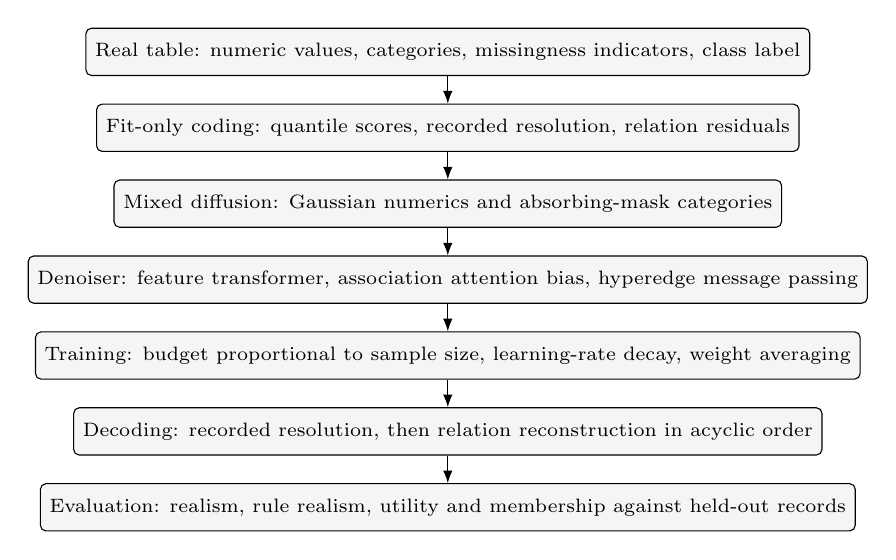
\begin{tikzpicture}[node distance=3.5mm, every node/.style={font=\scriptsize, align=center}, box/.style={draw, rounded corners=2pt, minimum width=7.6cm, minimum height=6mm, fill=gray!8}, arr/.style={-{Latex[length=1.6mm]}}]
\node[box] (a) {Real table: numeric values, categories, missingness indicators, class label};
\node[box, below=of a] (b) {Fit-only coding: quantile scores, recorded resolution, relation residuals};
\node[box, below=of b] (c) {Mixed diffusion: Gaussian numerics and absorbing-mask categories};
\node[box, below=of c] (d) {Denoiser: feature transformer, association attention bias, hyperedge message passing};
\node[box, below=of d] (e) {Training: budget proportional to sample size, learning-rate decay, weight averaging};
\node[box, below=of e] (f) {Decoding: recorded resolution, then relation reconstruction in acyclic order};
\node[box, below=of f] (g) {Evaluation: realism, rule realism, utility and membership against held-out records};
\foreach \x/\y in {a/b,b/c,c/d,d/e,e/f,f/g} \draw[arr] (\x) -- (\y);
\end{tikzpicture}
\caption{Overview of the corrected MedHyperDiff pipeline and its evaluation.}
\label{fig:pipeline}
\end{figure}

MedHyperDiff is a mixed-type diffusion model with Gaussian diffusion for numerical values, absorbing-mask diffusion for categories and explicit missingness indicators (Fig.~\ref{fig:pipeline}). Its denoiser is a feature transformer with an attention bias from a bootstrap-stable association graph and nonlinear hyperedge message passing over supplied clinical relations. A physical-unit rule energy is used in training and optionally as sampling guidance. Ten development iterations on four public UCI cohorts (Indian Liver Patient Dataset, heart failure, chronic kidney disease and early-stage diabetes) had produced partition-dependent effects and a repaired Gaussian copula that dominated the model on realism and rule compliance.

The audit found that 13 of 36 fits in one iteration stopped during the initial plateau of the validation loss and kept checkpoints from epochs 3 to 28, while the other 23 reached the 100-epoch cap still improving. Enzyme and bilirubin values were linearly scaled, every numerical column had a fixed reporting grid but outputs were continuous, an empirical protein tolerance was scored as if fewer violations were always better, and the TabDDPM adapter used a constant learning rate with early stopping instead of the upstream recipe. The modified implementation reproduces an archived synthetic table byte for byte under the original settings, so each correction can be isolated.

Table~\ref{tab:ablation} and Fig.~\ref{fig:ablation} apply the corrections one at a time on three development partitions of the liver dataset with three seeds each. The training correction alone reduced association error by 61\%, to the level of a control that simply resamples training rows, and restoring only the original checkpoint selection undid most of that gain. Decoding to the recorded resolution produced most of the remaining improvement in two-sample realism, measured as the AUROC of a classifier separating synthetic from real records, where 0.5 means indistinguishable.

\begin{table}[t]
\caption{Correcting one pitfall at a time (liver dataset, development partitions)}
\label{tab:ablation}
\centering
\setlength{\tabcolsep}{4pt}
\begin{tabular}{lcccc}
\toprule
Variant & C2ST & Num. W & Assoc. & Rule gap \\
\midrule
Original recipe & 0.855 & 0.245 & 0.176 & 0.004 \\
+ fixed-budget training & 0.730 & 0.167 & 0.068 & 0.006 \\
+ quantile coding, 100 steps & 0.714 & 0.151 & 0.066 & 0.006 \\
+ recorded resolution & \textbf{0.571} & \textbf{0.150} & \textbf{0.066} & \textbf{0.001} \\
All but original selection & 0.697 & 0.166 & 0.158 & 0.002 \\
Repaired copula & 0.573 & 0.153 & 0.079 & 0.006 \\
Bootstrap copy control & 0.493 & 0.150 & 0.066 & 0.002 \\
\bottomrule
\end{tabular}
\end{table}

\begin{figure*}[t]
\centering
\includegraphics[width=\textwidth]{figures/fig_ablation.png}
\caption{Effect of each correction on the liver dataset development partitions (mean and standard deviation across three partitions). C2ST is the two-sample classifier AUROC (0.5 is indistinguishable), numeric W the Wasserstein distance scaled by the training standard deviation, and the rule gap the difference between synthetic and real violation rates.}
\label{fig:ablation}
\end{figure*}

After correction, a pre-registered comparison with equal tuning budgets against upstream-recipe TabDDPM and TabDiff, CTGAN, TVAE and statistical references was evaluated once on reserved test folds. The corrected model improved on the original recipe in every seed and cohort, reducing two-sample AUROC from 0.944 to 0.631 on the liver data, from 0.761 to 0.615 on heart failure and from 0.782 to 0.586 on kidney disease. TabDiff and the copula were nevertheless more realistic overall. This stage also revealed the last two pitfalls: several TabDDPM configurations chosen by a fidelity and utility rule had membership AUROC between 0.91 and 0.99, and with 60 to 117 test patients the seed-to-seed standard deviation of the two-sample AUROC reached 0.07.

\section{Controlled Study Design}

The case study cannot separate the pitfalls from one model's idiosyncrasies or from the noise of small test folds. The controlled study, pre-registered before any generator was fitted to the new data, addresses both. It uses NHANES 2017 to 2018 \cite{nhanes} adults with a standard biochemistry record (4,756 records, diagnosed diabetes as label, 21 numerical predictors and sex), in which globulin equals total protein minus albumin and body mass index equals weight over squared height by definition, and the UCI thyroid registry (9,172 records, any thyroid diagnosis as label, six numerical and sixteen categorical predictors, up to 28\% missing), in which the free thyroxine index approximately equals total thyroxine divided by thyroid hormone uptake.

Each population is split once into a reference half and a pool half, grouped by identical predictor profile and stratified by label. From the pool, training samples of 250 and 1,000 records are drawn five times each and split 80/20 into fit and validation rows. All generators fit the same rows, and only early-stopping variants use the validation rows. The reference half, with 2,378 and 4,588 records, is never fitted and serves for utility, two-sample tests and as the source of non-members and attacker background data. Twelve variants are compared: corrected MedHyperDiff, the same with original early stopping or linear scaling, TabDDPM with the upstream recipe and with an earlier adapter loop, TabDiff, CTGAN, TVAE, a Gaussian copula, a copula with re-derivation of supplied relations, independent marginals, and bootstrap resampling as a copy control. Configurations are fixed in advance.

Every continuous-output generator emits raw values that are decoded after sampling in three ways using training rows only: raw, a single global grid per column, and a magnitude-banded grid. We compute two-sample AUROC with a random forest discriminator on the full reference and at 50 to 1,000 records per source with ten subsamples each, numerical and dependence distances, forest utility trained on synthetic and tested on real data, rule violation rates and rule realism, a nearest-distance membership attack and a density-ratio membership attack in the style of DOMIAS \cite{vanbreugel2023domias}. Rankings are compared by the fraction of generator pairs whose order reverses and by Kendall's $\tau$, with bootstrap intervals over the five training samples.

\section{Results of the Controlled Study}

\subsection*{Common Versus Corrected Practice}

We ranked eight generator identities under a common-practice pipeline, consisting of diffusion models trained with validation-loss early stopping, the adapter TabDDPM recipe, raw outputs, two-sample tests on 100 records per source and no privacy check, and under the corrected pipeline. Table~\ref{tab:pipeline} and Fig.~\ref{fig:pipeline_rev} show that a quarter to a third of all pairwise comparisons reversed and that the top-ranked generator changed in 18 of 20 training samples. The case-study model ranked fourth to sixth of eight under common practice in most samples and first in 16 of 20 under corrected practice.

\begin{table}[t]
\caption{Ranking agreement between common and corrected practice}
\label{tab:pipeline}
\centering
\setlength{\tabcolsep}{3pt}
\begin{tabular}{lcccc}
\toprule
Population, $n$ & Pairs reversed & $\tau$ & Top-1 agree & Top (corrected) \\
\midrule
NHANES, 250 & 32\% (29 to 35) & 0.36 & 0/5 & MedHyperDiff \\
NHANES, 1,000 & 34\% (29 to 38) & 0.33 & 0/5 & MedHyperDiff \\
Thyroid, 250 & 25\% (22 to 28) & 0.50 & 0/5 & MedHyperDiff \\
Thyroid, 1,000 & 26\% (22 to 31) & 0.47 & 2/5 & MedHyperDiff \\
\bottomrule
\end{tabular}
\end{table}

\begin{figure*}[t]
\centering
\includegraphics[width=\textwidth]{figures/pipeline_reversals.png}
\caption{Fraction of generator pairs whose order reverses between common and corrected practice, for realism, privacy-aware realism and rule scoring (mean and 95\% bootstrap interval over five training samples).}
\label{fig:pipeline_rev}
\end{figure*}

\subsection*{Training Choices}

With validation-loss early stopping, 30\% of MedHyperDiff fits kept a checkpoint from the first 20 epochs, the earliest at epoch 3, and 45\% stopped at the cap (Fig.~\ref{fig:epochs}). Two-sample AUROC was worse than with fixed-budget training on identical rows in all 20 paired samples, by 0.22 and 0.16 on NHANES and thyroid at 250 records and by 0.17 and 0.07 at 1,000 records, and association error was also worse in all 20. The earlier TabDDPM adapter loop on the upstream architecture diverged, with two-sample AUROC between 0.995 and 1.000 and utility between 0.49 and 0.70, against 0.74 to 0.91 and 0.87 to 0.94 with the upstream recipe. Quantile coding lowered two-sample AUROC relative to linear scaling in three of four settings, by 0.02 to 0.07 in every sample, but raised it by 0.03 for NHANES at 250 records, so the representation is a choice to validate rather than a fixed rule.

\begin{figure*}[t]
\centering
\includegraphics[width=0.9\textwidth]{figures/p1_selected_epochs.png}
\caption{Selected epoch as a fraction of the cap under validation-loss early stopping. The dashed line marks the first 20\% of training.}
\label{fig:epochs}
\end{figure*}

\subsection*{Recording Resolution}

Decoding changed some generators by up to 0.31 and others not at all (Table~\ref{tab:precision}, Fig.~\ref{fig:precision}). The difference lies in the inverse transforms rather than the models. TabDDPM and TabDiff invert quantile transforms whose tied knots return 45\% to 98\% of values exactly on the recording grid, which acts as an implicit decoding, whereas MedHyperDiff, TVAE and CTGAN emit almost no on-grid values. Without explicit decoding, rankings reversed for 29\% to 32\% of generator pairs on NHANES and 7\% to 14\% on thyroid, and the top generator changed. On the thyroid data, where hormone values are reported to about two significant figures, a single grid per column recovered only part of the effect.

\begin{table}[t]
\caption{Two-sample AUROC by decoding (training size 1,000)}
\label{tab:precision}
\centering
\setlength{\tabcolsep}{3pt}
\begin{tabular}{lccccc}
\toprule
& \multicolumn{2}{c}{NHANES} & \multicolumn{3}{c}{Thyroid} \\
Generator & Raw & Decoded & Raw & Global & Banded \\
\midrule
MedHyperDiff & 0.999 & 0.692 & 0.808 & 0.763 & 0.685 \\
TVAE & 0.991 & 0.913 & 0.950 & 0.947 & 0.934 \\
TabDiff & 0.703 & 0.703 & 0.698 & 0.696 & 0.692 \\
TabDDPM & 0.744 & 0.738 & 0.742 & 0.747 & 0.745 \\
\bottomrule
\end{tabular}
\end{table}

\begin{figure*}[t]
\centering
\includegraphics[width=\textwidth]{figures/p3_precision_c2st.png}
\caption{Two-sample AUROC against the reference population for raw outputs and outputs decoded to the recorded resolution (mean of five training samples).}
\label{fig:precision}
\end{figure*}

\subsection*{Rules and Memorization}

No learned generator reproduced the supplied relations. Between 90\% and 100\% of their NHANES records violated the definitional globulin or body mass index identities at recorded resolution, against 0\% in real data, and most thyroid records violated the free thyroxine envelope, against about 5\% in real data. Re-deriving definitional variables from their operands reproduced real behavior exactly. Scoring by violation counts rather than by the gap to real rates reversed 11\% to 22\% of generator pairs but not the winner.

Across generators, lower two-sample AUROC went with higher membership AUROC, with Spearman correlations between $-0.33$ and $-0.77$ (Fig.~\ref{fig:memo}). Excluding the copy control, the most realistic generator in a training sample exceeded a membership AUROC of 0.60 on at least one attack in 40\%, 0\%, 80\% and 20\% of samples for NHANES at 250 and 1,000 records and thyroid at 250 and 1,000 records. Upstream TabDDPM reached 0.85 to 0.89 at 250 records. In the case-study search over 160 configurations, the most realistic configuration of a method memorized in 10 of 20 cohort and method combinations.

\begin{figure*}[t]
\centering
\includegraphics[width=\textwidth]{figures/p6_memorization.png}
\caption{Realism against membership risk for each generator (mean of five training samples). Points above the dashed line exceed a membership AUROC of 0.60 on at least one of two attacks.}
\label{fig:memo}
\end{figure*}

\subsection*{Evaluation Size}

Table~\ref{tab:evalsize} and Fig.~\ref{fig:evalsize} report the probability that a single two-sample test orders a generator pair as the full reference does. At the 60 to 120 test patients typical of public clinical cohorts, about one comparison in six was ordered wrongly, and close competitors were separated little better than by chance. Agreement reached 90\% only at about 500 records per source.

\begin{table}[t]
\caption{Probability that one evaluation orders a pair correctly}
\label{tab:evalsize}
\centering
\setlength{\tabcolsep}{4pt}
\begin{tabular}{lccccc}
\toprule
Records per source & 50 & 100 & 200 & 500 & 1,000 \\
\midrule
NHANES & 0.77 & 0.85 & 0.88 & 0.93 & 0.96 \\
Thyroid & 0.78 & 0.84 & 0.90 & 0.94 & 0.95 \\
Pairs differing by at most 0.02 & 0.58 & 0.59 & 0.58 & 0.65 & 0.71 \\
Median single-draw SD & 0.062 & 0.045 & 0.031 & 0.015 & 0.008 \\
\bottomrule
\end{tabular}
\end{table}

\begin{figure}[t]
\centering
\includegraphics[width=\columnwidth]{figures/p7_evaluation_size.png}
\caption{Agreement between a single two-sample test and the full reference ordering as a function of evaluation size. The dashed line marks 90\%.}
\label{fig:evalsize}
\end{figure}

\section{A Generator That Preserves Laboratory Relationships}

The controlled study showed that learned generators break supplied laboratory relations, while the case study showed that exact enforcement over-corrects relations that real data satisfy only approximately. We therefore extended MedHyperDiff with relation reparameterization. For a relation linking several participants, one participant is reconstructed, and the generator models the remaining participants together with a residual equal to the reconstructed variable minus the value implied by the relation. After sampling, the generated columns are decoded to their recorded resolution, and each reconstructed variable is recovered as the implied value plus the learned residual. Exact and approximate relations are therefore handled alike, and rounding noise and rare discrepancies are reproduced rather than forced to zero or ignored. Each residual and its operands form a hyperedge of the model.

The choice of reconstructed participant matters. Reconstructing a narrow quantity, such as a small percentage or a tightly regulated index, from wide ones amplifies the errors of the generated operands. During development, reconstructing the basophil fraction or the mean corpuscular hemoglobin concentration raised two-sample AUROC to between 0.84 and 0.88. The final method chooses automatically from training rows one participant per relation such that an acyclic reconstruction order exists and the summed spread of reconstructed participants is largest, measured on the scale where the relation is additive, which is the logarithmic scale for products and ratios and the raw scale for sums and differences.

The method was tested on a population never used before, 4,865 NHANES adults with a complete blood count. The analyser measures red cell count, hemoglobin and mean corpuscular volume and computes hematocrit, mean corpuscular hemoglobin and mean corpuscular hemoglobin concentration, and the five white cell differential percentages sum to 100, all up to reporting rounding. The variant was chosen on a separate development pool with a pre-registered rule, then evaluated on a never-fitted reference half of 2,433 records with five training samples per size. Published generators were compared as generated, with hard derivation of the linked values, which corresponds to exact constraint enforcement, and with derivation plus resampled real residuals. The same reparameterization was also applied to TabDiff.

\begin{table}[t]
\caption{Blood count confirmation (mean of five samples; MedHyperDiff better in the number of samples shown)}
\label{tab:relation}
\centering
\setlength{\tabcolsep}{2.5pt}
\begin{tabular}{llcccc}
\toprule
$n$ & Measure & Ours & TabDiff & TabDiff+der. & TabDiff+rep. \\
\midrule
\multirow{4}{*}{250} & Relation dist. & \textbf{0.187} & 12.14 (5) & 0.965 (5) & 0.257 (5) \\
& C2ST & \textbf{0.691} & 0.762 (5) & 0.736 (5) & 0.745 (5) \\
& Utility AUROC & \textbf{0.717} & 0.670 (5) & 0.671 (5) & 0.679 (5) \\
& Membership & 0.555 & 0.619 & 0.618 & 0.598 \\
\midrule
\multirow{4}{*}{1,000} & Relation dist. & \textbf{0.173} & 3.92 (5) & 0.911 (5) & 0.184 (5) \\
& C2ST & 0.664 & 0.645 (1) & \textbf{0.633} (0) & 0.643 (0) \\
& Utility AUROC & 0.735 & 0.735 (2) & 0.733 (2) & 0.742 (1) \\
& Membership & 0.509 & 0.560 & 0.561 & 0.548 \\
\bottomrule
\end{tabular}
\end{table}

\begin{figure*}[t]
\centering
\includegraphics[width=\textwidth]{figures/relation_fidelity.png}
\caption{Reproduction of the four supplied blood count relations on the reference population (mean of five training samples, logarithmic scale). The highlighted point is MedHyperDiff with relation reparameterization.}
\label{fig:relation}
\end{figure*}

Table~\ref{tab:relation} and Fig.~\ref{fig:relation} summarize the confirmation. With 250 training records, the method reproduced the four relations better than TabDiff, TabDDPM, CTGAN, TVAE and the copula in all five samples, whether these were used as generated, with relation distances between 12 and 244, or with hard derivation, with distances between 0.95 and 0.97. It also beat derivation with resampled real residuals in four of five samples. At the same time it was the most realistic generator that did not copy patients, with a two-sample AUROC of 0.691 against 0.731 for the best published alternative, and the most useful for prediction, with an AUROC of 0.717 against at most 0.687 for non-memorizing published alternatives, while its membership AUROC was 0.555. All pre-registered criteria for the claim were met at this size. With 1,000 training records the relation advantage persisted in all five samples, but TabDiff became more realistic overall, with a two-sample AUROC of 0.633 after hard derivation against 0.664, so the full claim was not supported at that size. This configuration used the same 5,000 optimizer steps at every sample size, which the next section shows to be the cause.

\section{Robustness Across Populations, Relations and Sizes}

A result on one population and one family of relations could be specific to that setting. We therefore ran a second pre-registered study with four questions: whether the relation advantage replicates on independent populations, whether it extends to relations of a different kind, where TabDiff overtakes the model as the training size grows, and whether relation reparameterization also helps other generators when added to them.

\subsection*{Design}

Six new NHANES populations were built from the public files of four survey cycles. Blood count populations from 2013 to 2014 (5,229 adults) and 2021 to 2023 (5,555 adults) carry the four approximate relations above. Chemistry populations from 2011 to 2012 (4,778 adults) and 2021 to 2023 (5,284 adults) contain 20 numerical variables from anthropometry, the standard biochemistry profile and urine tests, with four relations that NHANES computes from reported values: globulin as total protein minus albumin, body mass index, the urine albumin to creatinine ratio, and calculated serum osmolality, $1.86\,\text{Na} + \text{glucose}/18 + \text{BUN}/2.8 + 9$. An audit before any fitting showed that every chemistry relation holds exactly at reported precision, whereas no blood count relation does. For relations of this kind the decoder re-derives the reported value from the decoded operands after reconstruction, as the laboratory does, and hard derivation is already the correct post-processing, so for them we test non-inferiority to hard derivation rather than superiority. Populations from 2015 to 2016 served only for development.

The training budget was the one change to the model. Four candidates were fixed in advance: the previous configuration, optimizer steps proportional to the sample size so that the number of passes over the data is constant, and two variants that also widened the network. On development data the proportional budget with the original width lowered the mean two-sample AUROC from 0.690 to 0.653, whereas wider networks did not help and increased membership risk, and the pre-registered rule selected it. Confirmation used the never-fitted reference half of each population, training sizes of 250 and 1,000 records with five samples each, and 2,000 records with three samples in the two newest populations. A smaller size of 100 records was removed during the run by a recorded amendment, before any comparator result was examined. All published generators were evaluated as generated, with hard derivation and with derivation plus resampled residuals, and each was also fitted with relation reparameterization added. In total 608 confirmation fits completed without failure.

\subsection*{Relation Fidelity}

The relation advantage replicated everywhere (Table~\ref{tab:robust}, Fig.~\ref{fig:robust_rel}). In both blood count populations and at all three sizes the model reproduced the relations better than every published generator, as generated and with hard derivation, in every training sample. Hard derivation over-corrected the approximate relations by a factor of about seven, and TabDiff as generated missed them by one to two orders of magnitude. For the exact chemistry relations the model was better than every generator as generated in every sample and also lower than the best hard-derived generator in every setting. Derivation with resampled real residuals came close, and on the 2011 to 2012 chemistry population it was slightly better, with distances of 0.045 and 0.019 against 0.049 and 0.025.

\begin{table}[t]
\caption{Confirmation on four new populations (mean over samples). Comparators are the best published generator in any processing whose membership AUROC is at most 0.60}
\label{tab:robust}
\centering
\setlength{\tabcolsep}{2.2pt}
\begin{tabular}{llcccccc}
\toprule
& & \multicolumn{2}{c}{Relation dist.} & \multicolumn{2}{c}{C2ST} & \multicolumn{2}{c}{Utility} \\
Population & $n$ & Ours & Hard der. & Ours & Best & Ours & Best \\
\midrule
Blood 2013--14 & 250 & \textbf{0.128} & 0.743 & \textbf{0.709} & 0.728 & \textbf{0.709} & 0.698 \\
& 1,000 & \textbf{0.092} & 0.741 & 0.646 & \textbf{0.634} & \textbf{0.771} & 0.753 \\
Blood 2021--23 & 250 & \textbf{0.151} & 0.968 & \textbf{0.690} & 0.719 & \textbf{0.684} & 0.680 \\
& 1,000 & \textbf{0.137} & 0.972 & \textbf{0.629} & 0.634 & \textbf{0.733} & 0.723 \\
& 2,000 & \textbf{0.136} & 0.974 & 0.616 & \textbf{0.577} & 0.745 & 0.745 \\
Chem. 2011--12 & 250 & \textbf{0.049} & 0.295 & \textbf{0.715} & 0.737 & \textbf{0.878} & 0.864 \\
& 1,000 & \textbf{0.025} & 0.284 & \textbf{0.644} & 0.674 & 0.888 & 0.888 \\
Chem. 2021--23 & 250 & \textbf{0.050} & 0.360 & \textbf{0.775} & 0.783 & \textbf{0.895} & 0.882 \\
& 1,000 & \textbf{0.025} & 0.354 & \textbf{0.700} & 0.749 & 0.904 & \textbf{0.905} \\
& 2,000 & \textbf{0.021} & 0.351 & 0.645 & \textbf{0.625} & 0.905 & \textbf{0.906} \\
\bottomrule
\end{tabular}
\end{table}

\begin{figure*}[t]
\centering
\includegraphics[width=\textwidth]{figures/relation_by_size.png}
\caption{Relation residual distance on the four confirmation populations by training size (mean and standard deviation over samples, logarithmic scale).}
\label{fig:robust_rel}
\end{figure*}

\begin{figure*}[t]
\centering
\includegraphics[width=\textwidth]{figures/c2st_by_size.png}
\caption{Two-sample AUROC on the four confirmation populations by training size (mean and standard deviation over samples). The dashed line is the model with the fixed budget of the earlier study.}
\label{fig:robust_c2st}
\end{figure*}

\subsection*{Realism, Utility and Training Size}

With 250 training records the model had the lowest two-sample AUROC of all generators that did not copy patients in all four populations, and the pre-registered criterion held in three of four, the exception being the 2011 to 2012 chemistry population, where its membership AUROC of 0.608 exceeded the 0.60 threshold. With 1,000 records it was within 0.02 of the most realistic generator in all four populations and the most realistic in three. Pooled over populations and samples, its two-sample AUROC was lower than that of the best published generator of each setting by 0.020 (95\% bootstrap interval 0.011 to 0.028) at 250 records and by 0.021 (0.008 to 0.033) at 1,000 records, and its utility AUROC was higher by 0.015 (0.010 to 0.020) and 0.012 (0.008 to 0.017). With 2,000 records TabDiff was more realistic, by 0.039 on blood counts and 0.020 on chemistry, with equal utility, so the crossover in realism lies between 1,000 and 2,000 training records (Fig.~\ref{fig:robust_c2st}). The budget explains the earlier result: with the fixed budget the model's two-sample AUROC barely changed between 1,000 and 2,000 records, whereas with the proportional budget it fell with every increase in data. Applied to the original blood count population, whose reference half had already been examined and which is therefore a secondary check, the proportional budget reversed the earlier failure at 1,000 records, with a two-sample AUROC of 0.627 against 0.633 for TabDiff with hard derivation.

\subsection*{Reparameterization as a Plug-In}

Added to the strong published generators, relation reparameterization reliably repaired their relations. For TabDiff, TabDDPM and the copula it lowered the relation distance relative to the raw output in every setting and matched or beat hard derivation, usually without loss of realism. It is not a universal plug-in, however, and the pre-registered claim that it helps every generator was not supported, holding in 37 of 50 generator and setting combinations. CTGAN and TVAE generate implausible operands on the chemistry panel, such as urine creatinine near zero, which no post-processing can turn into a faithful ratio, and TabDiff with reparameterization was unstable in one sample at 2,000 records, with a two-sample AUROC of 0.88.

\section{A Corrected Protocol}

The results suggest a corrected protocol with seven elements. Diffusion models should be trained with a fixed optimization budget chosen during development and scaled with the training size, with learning-rate decay and weight averaging, and any validation-based selection should report the selected epochs. The numerical representation should be validated rather than assumed. Every continuous-output generator should be decoded to the recorded resolution, per order of magnitude where reporting uses significant figures, and the on-grid fraction of raw outputs should be reported. Definitional variables should be re-derived, and approximate relations should be scored against real held-out behavior through the violation-rate gap and the residual distance. Baselines should be run with their upstream training loops. Membership inference with at least a nearest-distance attack, a density-ratio attack and a copy control should accompany every realism metric, and configurations should be selected under a privacy constraint. Two-sample tests should use about 500 or more records per source where possible, with repeated subsampling, and differences below 0.02 should be treated as unresolved.

\section{Discussion}

The seven pitfalls share one property: each changes which generator appears best without any change to the distributions the generators have learned. Validation-loss selection and non-upstream baseline loops change what is trained, inverse-transform details decide whether raw outputs land on the recording grid, violation counts and two-sample tests reward over-correction and copying, and small evaluation sets add enough noise to reorder close competitors. Together they reversed a quarter to a third of all comparisons in a controlled setting and most conclusions of a ten-iteration development project.

The relation study shows the constructive side of trustworthy evaluation. Once evaluation is reliable, a targeted mechanism can be shown to help in a precisely stated setting and not in others. Small clinical datasets with known laboratory relationships are common, since rare diseases, single-site cohorts, pediatric studies and most public clinical tables contain hundreds rather than thousands of patients, and large datasets are often split into small subgroups. Across five independent populations, two families of relations and training sizes up to 1,000 records, the proposed model offers the most faithful, realistic and useful synthetic data among the generators tested, without memorization. This range covers most clinical data-sharing requests. With about 2,000 records or more TabDiff is more realistic overall, so the practical recommendation depends on the use: when laboratory relations must hold, as in synthetic data used to develop clinical rules or to teach, the proposed model remains preferable because TabDiff misses the relations by at least an order of magnitude and exact derivation over-corrects approximate ones. A simple post-processing that adds resampled real residuals approaches the relation fidelity of our model at no cost and should be standard practice for any generator. The second study also shows the value of the corrected protocol a second time: the earlier negative result at 1,000 records came from a training budget that did not scale with the data, a variant of the first pitfall.

\section{Limitations}

The controlled study uses two populations, one NHANES cycle without survey weights, fixed default configurations, two training sizes and five training samples drawn from a common pool, so intervals reflect training-sample variation only. The relation studies use only NHANES populations, without survey weights, and fixed comparator configurations rather than tuned ones. The results at 2,000 records rest on three overlapping samples in two populations, and the 100-record condition was removed by amendment, so the smallest samples remain untested. Three disclosed development rounds in the first relation study make its development estimates optimistic, although not its confirmation. Membership attacks are empirical diagnostics, the threshold of 0.60 is a convention, and no formal privacy guarantee is claimed. TabDDPM and TabDiff are adaptations of pinned upstream code rather than reproductions of their published benchmarks. All computations used CPUs under variable background load.

\section{Conclusion}

Routine training and evaluation choices can determine which synthetic data generator appears best on small clinical tables. Correcting seven such choices reversed a quarter to a third of generator comparisons in a pre-registered controlled study. Using the corrected protocol, relation reparameterization allowed a hypergraph-guided diffusion model to reproduce laboratory relationships better than published generators on five independent populations and two families of relations, and with a training budget proportional to the sample size it was also the most realistic and useful generator that did not copy patients up to 1,000 training records. TabDiff remains more realistic with larger samples. Code, hashed run records, protocols and reports are released to allow every number in this paper to be reproduced.

\section*{Acknowledgment}

We thank the National Center for Health Statistics for NHANES, the Garvan Institute and Ross Quinlan for the thyroid data, and the UCI Machine Learning Repository.

\begin{thebibliography}{00}
\bibitem{xu2019ctgan} L. Xu, M. Skoularidou, A. Cuesta-Infante, and K. Veeramachaneni, ``Modeling tabular data using conditional GAN,'' in \textit{Advances in Neural Information Processing Systems}, 2019.
\bibitem{ho2020ddpm} J. Ho, A. Jain, and P. Abbeel, ``Denoising diffusion probabilistic models,'' in \textit{Advances in Neural Information Processing Systems}, 2020.
\bibitem{austin2021d3pm} J. Austin, D. D. Johnson, J. Ho, D. Tarlow, and R. van den Berg, ``Structured denoising diffusion models in discrete state-spaces,'' in \textit{Advances in Neural Information Processing Systems}, 2021.
\bibitem{kotelnikov2023tabddpm} A. Kotelnikov, D. Baranchuk, I. Rubachev, and A. Babenko, ``TabDDPM: Modelling tabular data with diffusion models,'' in \textit{Proc. Int. Conf. Machine Learning}, 2023.
\bibitem{shi2025tabdiff} J. Shi, M. Xu, H. Hua, H. Zhang, S. Ermon, and J. Leskovec, ``TabDiff: A mixed-type diffusion model for tabular data generation,'' in \textit{Proc. Int. Conf. Learning Representations}, 2025.
\bibitem{liu2023goggle} T. Liu, Z. Qian, J. Berrevoets, and M. van der Schaar, ``GOGGLE: Generative modelling for tabular data by learning relational structure,'' in \textit{Proc. Int. Conf. Learning Representations}, 2023.
\bibitem{stoian2024cdgm} M. C. Stoian, S. Dyrmishi, M. Cordy, T. Lukasiewicz, and E. Giunchiglia, ``How realistic is your synthetic data? Constraining deep generative models for tabular data,'' in \textit{Proc. Int. Conf. Learning Representations}, 2024.
\bibitem{stoian2025drl} M. C. Stoian and E. Giunchiglia, ``Beyond the convexity assumption: Realistic tabular data generation under quantifier-free real linear constraints,'' arXiv:2502.18237, 2025.
\bibitem{shankar2026harpoon} Shankar \textit{et al.}, ``Harpoon,'' in \textit{Proc. Int. Conf. Learning Representations}, 2026. [Online]. Available: https://openreview.net/forum?id=G5g6tDg1ZE
\bibitem{lopezpaz2017c2st} D. Lopez-Paz and M. Oquab, ``Revisiting classifier two-sample tests,'' in \textit{Proc. Int. Conf. Learning Representations}, 2017.
\bibitem{vanbreugel2023domias} B. van Breugel, H. Sun, Z. Qian, and M. van der Schaar, ``Membership inference attacks against synthetic data through overfitting detection,'' in \textit{Proc. Int. Conf. Artificial Intelligence and Statistics}, 2023.
\bibitem{giomi2023anonymeter} M. Giomi, F. Boenisch, C. Wehmeyer, and B. Tasn\'adi, ``A unified framework for quantifying privacy risk in synthetic data,'' \textit{Proc. Privacy Enhancing Technologies}, 2023.
\bibitem{bengio2004variance} Y. Bengio and Y. Grandvalet, ``No unbiased estimator of the variance of k-fold cross-validation,'' \textit{J. Machine Learning Research}, vol. 5, pp. 1089--1105, 2004.
\bibitem{nhanes} National Center for Health Statistics, ``National Health and Nutrition Examination Survey data files, cycles 2011--2012 to August 2021--August 2023,'' Centers for Disease Control and Prevention, 2013--2024.
\end{thebibliography}

\end{document}
